\documentclass[letter]{article}
\renewcommand{\baselinestretch}{1.25}

\usepackage[margin=1in]{geometry}
\usepackage{physics}
\usepackage{amsmath, mathtools}
\numberwithin{equation}{section}
\usepackage{amssymb}
\usepackage{graphicx}
\usepackage{hyperref}
\usepackage{empheq}

% MATLAB Formating Code
\usepackage[numbered,framed]{matlab-prettifier}
\lstset{style=Matlab-editor,columns=fullflexible}
\renewcommand{\lstlistingname}{Script}
\newcommand{\scriptname}{\lstlistingname}

% Document Specific
\newcommand{\sat}{\text{sat}}
\newcommand{\sign}{\text{sign}}

\allowdisplaybreaks

%opening
\title{MECH 6313 - HW 7}
\author{Jonas Wagner}
\date{2021, May 14}

\begin{document}
	
	
%%%%%%%%%%%%%%%%%%%%%%%%%%%%%%%%%%%%%%%%%%%%%%%%%%%%%%%%%%%%%%%%%%%%%%%%%%%%%%
FUTURE VIEWER:
This assignment was never completed (or really worked on that much)
as it wasn't necessary since my lowest HW score would be dropped.
Sorry that it isn't of use to you... 
%%%%%%%%%%%%%%%%%%%%%%%%%%%%%%%%%%%%%%%%%%%%%%%%%%%%%%%%%%%%%%%%%%%%%%%%%%%%%%
	

\maketitle

\tableofcontents

%----------------------------------------------------------------------------
\newpage
\section{Problem 1}
\textbf{Problem:}
Using the PR Lemma, show that positive real linear systems
\begin{equation}
	\begin{aligned}
		\dot{x} &= Ax + Bu\\
		y &= Cx
	\end{aligned}
\end{equation}
which are known to also have a relative degree of one ($CB \neq 0$), also have a minimum phase property.\\

\noindent
\textbf{Solution:}
% Write system in Normal form then aply PR Lemma









\newpage
\section{Problem 2:}
The dynamics of a translational oscillator with a rotating actuator (TORA) are described by:
\begin{equation}
	\begin{aligned}
		\dot{x}_1 &= x_2\\
		\dot{x}_2 &= \cfrac{-x_1 + \epsilon x_4^2 \sin(x_3)}{1 - \epsilon^2 \cos[2](x_3)} + \cfrac{- \epsilon \cos(x_3)}{1 - \epsilon^2 \cos[2](x_3)} u\\
		\dot{x}_3 &= x_4\\
		\dot{x}_4 &= \cfrac{1}{1-\epsilon^2 \cos[2](x_3)} \qty(\epsilon \cos(x_3) \qty(x_1 - \epsilon x_4^2 \sin(x_3)) + u)
	\end{aligned}
\end{equation}
where $x_1$ and $x_2$ are the displacement and velocity of the platform, while $x_3$ and $x_4$ are the angle and angular velocity of the rotor. The rotor is carrying mass $m$ and a control torque of $u$ is applied to the rotor while the parameter $\epsilon > 1$ depends on the eccentricity $e$ and the masses $m$ and $M$.\\

\begin{figure}[h]
	\centering
	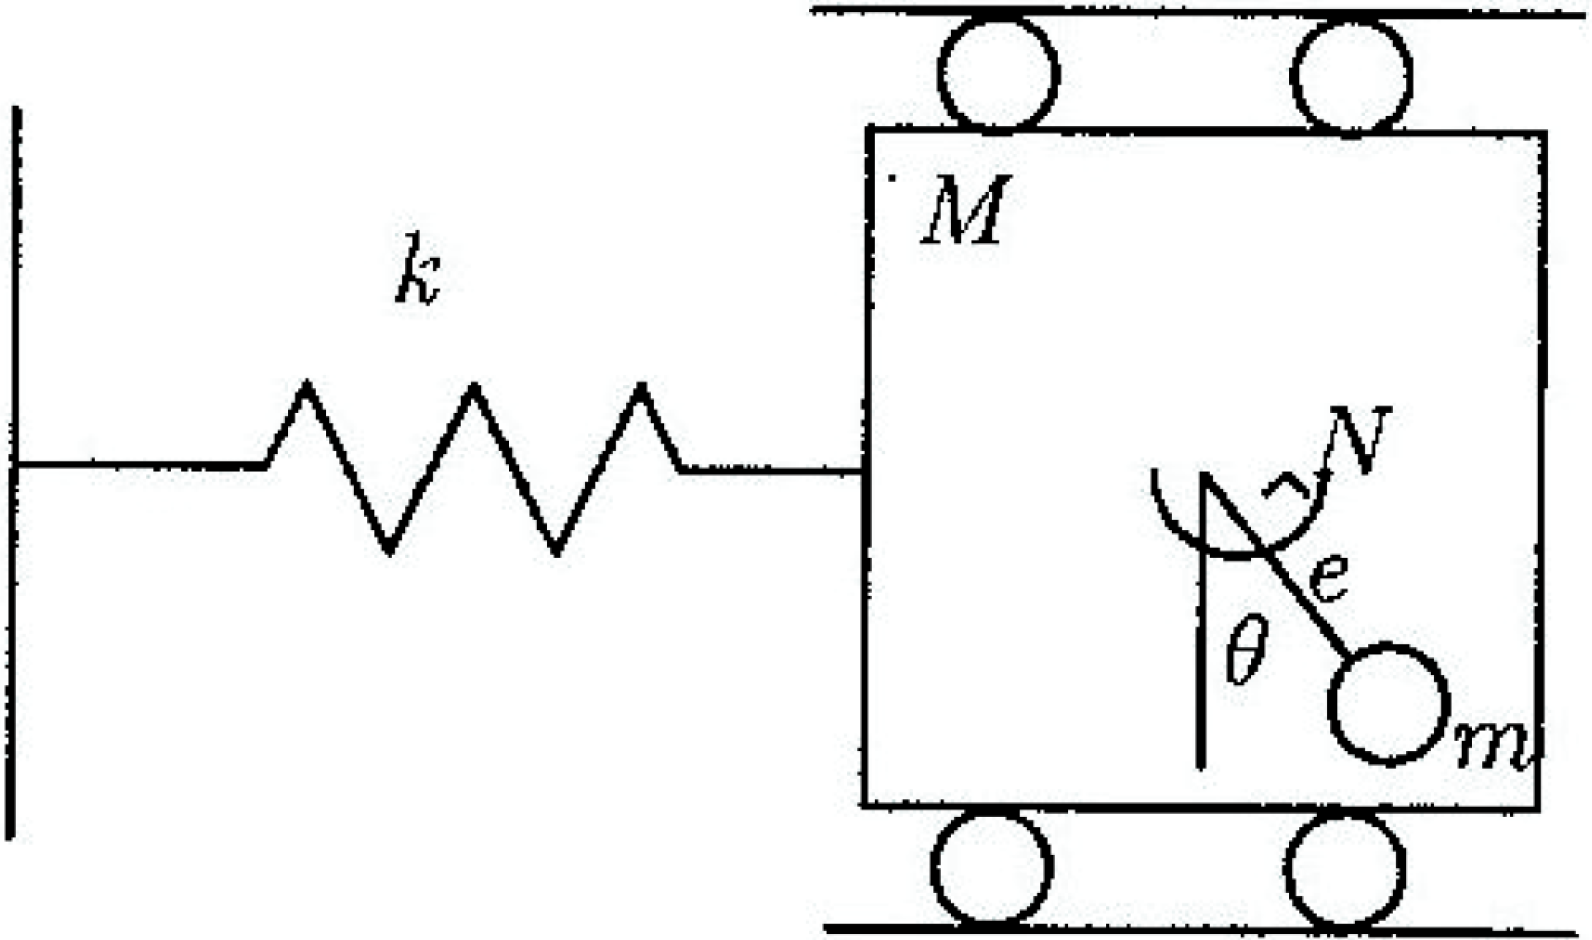
\includegraphics[width=0.7\linewidth]{fig/pblm2_fig}
	\caption{TORA system diagram}
	\label{fig:pblm2fig}
\end{figure}

\noindent
\textbf{Problem:}
With the output $y = x_3$ being the measurement of the rotor angular position, determine the relative degree and the zero dynamics. Also provide a physical interpretation of the zero dynamics.\\

\noindent
\textbf{Solution:}






\newpage
\section{Problem 3: Khalil P13.27}
The magnetic suspension system is modeled by
\begin{equation}
	\begin{aligned}
		\dot{x}_1 &= x_2\\
		\dot{x}_2 &= g - \frac{k}{m} x_2 - \cfrac{L_0 a x_3^2}{2m (a + x_1)^2}\\
		\dot{x}_3 &= \frac{1}{L(x_1)} \qty[-R x_3 + \frac{L_0 a x_2 x_3}{(a + x_1)^2} + u]
	\end{aligned}
\end{equation}
where $x_1 = y$, $x_2 = \dot{y}$, $x_3 = i$, and $u = v$.\\
Use the following numerical data:\\
$m = 0.1$ kg, $k = 0.01$ N/m/sec, $g = 9.81$ m/s$^2$, $a = 0.05$ m, $L_0 = 0.01$ H, $L_1 = 0.02$ H, and $R = 1 \ \Omega$.

\subsection{Part a}
\textbf{Problem:}
Show that the systems is feedback linearizable.\\

\noindent
\textbf{Solution:}








\subsection{Part b}
\textbf{Problem:}
Using feedback linearization, design a state feedback control law to stabilize the ball at $y = 0.05$ m.\\

\noindent
\textbf{Solution:}










\subsection{Part c}
\textbf{Problem:}
Show that when $y = x_1$, the system is input-output linearizable.\\

\noindent
\textbf{Solution:}







\subsection{Part d}
\textbf{Problem:}
Using feedback linearization, design a state feedback control law so that the output $y$ asymptotically tracks $r(t) = 0.05 + 0.01 \sin(t)$ and simulate the closed-loop system.\\

\noindent
\textbf{Solution:}











\newpage
\appendix
\section{MATLAB Code:}\label{apx:matlab}
All code I write in this course can be found on my GitHub repository:\\
\href{https://github.com/jonaswagner2826/MECH6313}{https://github.com/jonaswagner2826/MECH6313}
% MECH6313_HW7
%\lstinputlisting[caption={MECH6313\_Exam},label={script:Exam}]{MECH6313_Exam.m}


\end{document}
